%\newpage
\chapter{Fundamentação Teórica}

  
\section{Avaliação Docente do Instituto Federal de Goiás}
    O Instituto Federal de Goiás dispõe da Comissão Permanente de Pessoal Docente, como responsável pelas avaliações de desempenho para fins de progressão e promoção funcional, formada por 9 membros pertencentes ao quadro de servidores do IFG (Atualizado em 19 de agosto de 2021). Atualmente a CPPD é responsável por cerca de 1300 docentes que são avaliados periodicamente \cite{ifg}.
    
    A solução será importante para o processo de avaliação docente, pois essas avaliações impactam diretamente na progressão de carreira do docente. No cenário atual o SAD será necessário na automatização do processo diminuindo a margem de erros, pois atualmente as avaliações são feitas em sistemas distintos e vinculados a uma planilha, tornando-se um procedimento manual passível a falhas. 
    
    Logo ao gerar os dados no SAD existirá um processo de armazenamento centralizado de dados uma forma de consulta simples, pois estará disponível para visualização em um sistema Web, sendo que método atual, caso seja necessário por diversos motivos a busca de uma nota feita anteriormente, é um meio mais difícil pois é necessário a solicitação para a CPPD da planilha que está armazenada a nota.
    
    A solução atenderá a princípio toda a organização do IFG que contempla 14 campus, que atualmente possui como método a Ficha de Avaliação de Desempenho. A avalição é feita em dois períodos ao ano, de acordo com a Res. Consup IFG nº 040/2018, Regimento Geral do IFG, Art. 190-193,198-201, avaliando a atuação dos Docente, Coordenadores de Curso, Coordenador Acadêmico e Chefe de Departamento, atribuindo-lhe nota numa escala de 0(zero) à 10(dez). São feitas três avaliações a avaliação do aluno, a avaliação do chefe departamento ou coordenador de curso e a auto avaliação, gerando uma média aritmética com a nota do docente, que é necessário a soma das três notas e dividivizão pela soma das quantidades, um processo simples, porém a aplicação se torna bastante necessário e modificará o processo para melhor.


\section{Gerenciamento de Requisitos de Software}
  
    Conforme reuniões com os atuais membros pertencentes da comissão da CPPD, foram levantados os pontos necessários para o projeto do sistema para avaliação de desempenho docente. Serão realizadas reuniões para se possa ser feito as interações e troca de informações que poderão ser importantes para as decisões do projeto em questão. A abordagem visará que a CPPD colabore durante a etapa de análise de requisitos, mantendo todos alinhados com a solução, sendo uma maneira fácil para adoção, garantido a organização e eficiência.
    
    Na sequência foram elaborados alguns diagramas, a fim de facilitar o entendimento do sistema e facilitar o desenvolvimento. Pode-se visualizar no diagrama de caso de uso, os atores representados, identificando os usuários do sistema, que diferenciam seus papeis e níveis de acesso, servido como um unificador em todo o desenvolvimento do sistema.
    
    
    \begin{figure}[h]
    \centering
    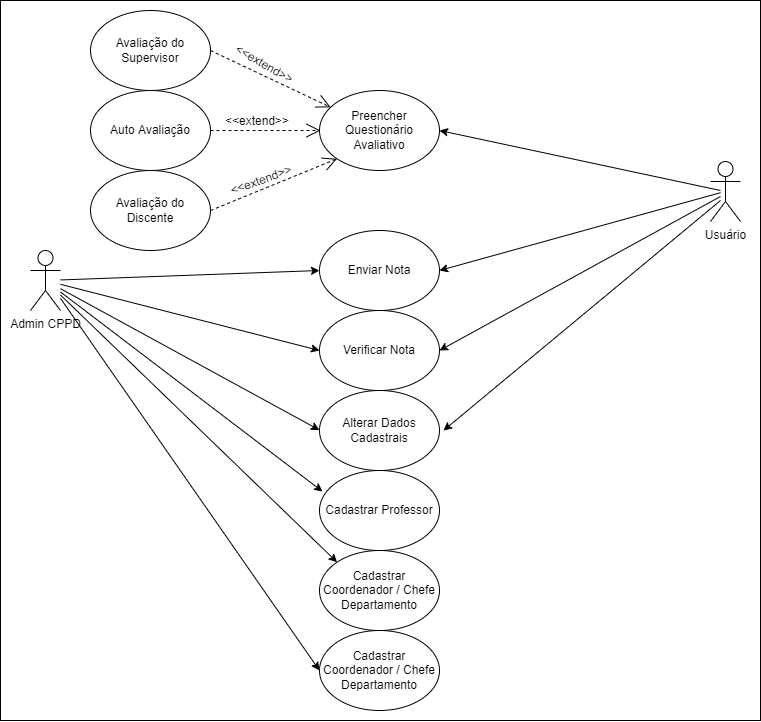
\includegraphics[width=0.55\textwidth]{./img/CasoUso.png}
    \caption{Diagrama de Caso de Uso}
    \label{fig:CasoUso}
    \end{figure}
    
    Segundo \citen{centenaro} o diagrama de caso de uso abaixo documenta o que o sistema faz da perspectiva do usuário. Em outras palavras, descreve as principais funções do sistema e as interações dessas funções com os usuários. Neste diagrama, não será aprofundando nos detalhes técnicos, informando como o sistema funciona.
    
    Baseado no que está sendo demostrado no diagrama de caso de uso, o sistema necessitará de funções que atenderam o cadastro de usuário, diferenciando seus privilégios e uma função para que possa ser preenchido, estruturado e consultado os questionários avaliativos.
    
    
\section{Metodologia Agil}

    Baseando-se na metodologia ágil, no \textit{framework Scrum}, onde as tarefas são reunidas em um  \textit{backlog}, e o projeto é dividido em blocos fixos de tempo com suas próprias tarefas e metas, ou seja, os sprints, serão divididas as etapas de desenvolvimento do projeto. Outro ponto bastante utilizado da metodologia ágil aplicada, onde será suficiente apenas ter um \textit{backlog} com as entregas pendentes do projeto, uma forma simples, pois o foco será em antecipar o máximo possível o trabalho \cite{juliana}.
    
    Durante o desenvolvimento do produto, serão definidas as etapas divididas em \textit{sprint}, conforme abordado por \citen{cronapp} “Um \textit{sprint backlog} é um tempo predeterminado que define o ciclo de desenvolvimento de um  \textit{software}”. Cada \textit{sprint} precisará ser validado, a parti da validação será iniciado uma novo \textit{backlog} do sistema. 
    
    Também será utilizado o sistema \textit{Planner}, conforme recomendações \textit{kamban}, para que consiga efetuar o controle por meio dos recursos de \textit{checklist} disponíveis, concentrando principalmente no gerenciamento das tarefas do ambiente de desenvolvimento.
        
        
\subsection{Scrum}

     Segundo \citen{scrum} o \textit{Scrum} é um método ágil para gestão de projetos. Ele é muito utilizado em equipes de desenvolvimento de software porque reúne um conjunto de boas práticas que facilitam o trabalho em equipes dessa natureza, como reuniões periódicas, lista de requisitos a serem atendidos, \textit{feedbacks} constantes sobre o produto, entre outros.
    
    O \textit{Scrum} é extremamente prescritivo, ou seja, para que um projeto dê certo dentro desse método é preciso seguir suas principais recomendações à risca, já que o Scrum define desde os papéis dentro da equipe de trabalho até a duração ideal das reuniões \cite{kamban}.
    
    No \textit{Scrum} exige que seja identificada uma lista de funcionalidades que precisam ser desenvolvidas para que o produto chegue ao objetivo esperado, o chamado \textit{Product Backlog}. Essa lista é traduzida em \textit{Sprints}: ciclos de tempo onde pequenas partes do produto são planejadas, executadas e entregues, e é justamente aí que o \textit{kanban} pode entrar como um facilitador.
    
    
\subsection{Kamban}

    De acordo com \citen{digite} o \textit{Kanban} é um sistema de gestão visual para controle de tarefas e fluxos de trabalho através da utilização de colunas e cartões, facilitando a gestão de atividades. Sendo muito comum confundir o \textit{kanban} com o \textit{Scrum}, ou achar que o \textit{Scrum} necessariamente precisa do \textit{kanban} para funcionar, mas não é bem assim.   
    
    O \textit{kanban} é um sistema, ou seja, uma ferramenta para auxiliar no trabalho da equipe, como uma linguagem de programação, por exemplo. Ele não é prescritivo ou impõe regras para que o trabalho seja feito corretamente, apenas possibilita que o time de trabalho execute suas tarefas com mais clareza e colaboração. E é por isso que, obviamente, o \textit{kanban} não funciona como um substituto para o \textit{Scrum}, no entanto, se utilizados juntos podem formar um casamento perfeito \cite{kamban}.
    
    No \textit{kanban} pode incorporar as \textit{Sprints} e traduzir todo o trabalho que precisa ser executado em cartões, facilitando a gestão das tarefas para agilizar as entregas e garantir autonomia ao time de desenvolvimento, que pode atribuir as próprias tarefas, princípios tão importantes para que o \textit{Scrum} funcione da melhor maneira.
    

\section{API RESTful com Java 8 e Spring Boot}

    O mercado de desenvolvimento tem avançado e apresentado inúmeros recursos e padrões novos, que devem ser seguidos para atender a demanda de acessos e dados que precisam manipular nos dias de hoje. \textit{APIs Restful} se tornaram peça chave para criação de aplicações robustas, seguindo padrões de micro serviços, além de trabalharem de modo \textit{standalone}, ou seja, sem que uma requisição dependa de outra para executar uma determinada operação \cite{souza}.

    Foi utilizado o recurso de criar as tabelas do banco de dados de modo automático, auxiliando até mesmo a criação das tabelas para os membros da equipe de desenvolvimento da mesma maneira. O \textit{Flyway} é um \textit{framework} que permite o controle de versão e automação durante a criação do banco de dados que pode-se configurar a criação de tabelas, os dados iniciais que devem estar na base de dados assim por diante. Também possui um utilitário de linha de comando que permite criar, atualizar e até mesmo limpar bancos de dados, tornando o gerenciamento de bancos de dados simples e intuitivo.

   Conforme \cite{vale} ao armazenar as senhas dos usuários a aplicação utiliza um modo seguro no banco de dados, utilizando o \textit{BCrypt} que permite encriptar irreversivelmente um certo valor, o que é ideal para armazenar informações com segurança em um banco de dados. O mais interessante é que, se chamado várias vezes, o \textit{BCrypt} criará diferentes valores de \textit{hash} para o mesmo valor, o que torna sua criptografia muito eficiente e segura, sendo a função \textit{hash} um algoritmo matemático para a criptografia, na qual ocorre uma transformação do dado (como um arquivo, senha ou informações) em um conjunto alfanumérico com comprimento fixo de caracteres.
    
%    Manter a lógica da  aplicação isolada e organizada em um só local, para que ela seja de fácil manutenção, e possa ser facilmente acessada por outros componentes.O Spring possui uma anotação chamada ‘Service’, que quando uma classe Java é anotada com ela, a mesma passará a ser um componente Spring. Esse componente Spring, deverá conter uma lógica de negócio específica, e poderá ser injetada como dependência de qualquer outro componente usando a anotação Autowired.
    
    Logo é apresentado os componentes \textit{Spring} como sendo serviços \textit{Restful}, o \textit{Spring Rest} possui a anotação \textit{Controller} que uma vez adicionada a uma classe Java, aceitará um \textit{path} como parâmetro, tornando esse componente disponível para acesso HTTP para o \textit{path} adicionado. Com os \textit{controllers}, também é possível gerenciar os verbos HTTP (GET, POST, PUT, DELETE,...) para cada método da classe, permitindo criar todos os acessos Restful para a API.
   
    Para expor uma API com o Spring Boot, a primeira coisa a fazer é adicionar a dependência do \textit{Spring Boot Web}, para isso foi adicionado ao arquivo pom.xml:
    

    \begin{figure}[h]
    \centering
    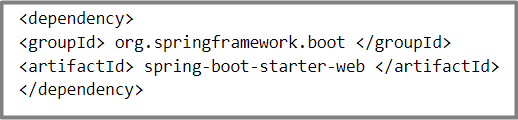
\includegraphics[width=0.55\textwidth]{./img/Dependência.png}
    \caption{Dependência Adicionas}
    \label{fig:Dependência}
    \end{figure}
    
    Após salvar o arquivo para instalar as dependências, que incluem o \textit{Tomcat, Jackson,} entre outras. Depois, foi criado uma classe Java com o seguinte código:
    
    \begin{figure}[h]
    \centering
    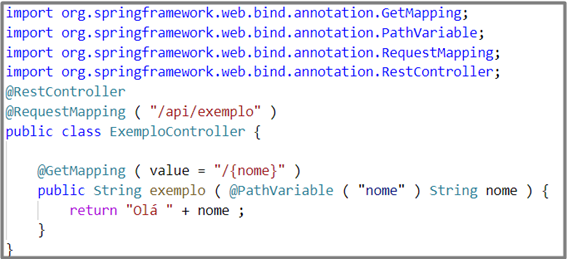
\includegraphics[width=0.60\textwidth]{./img/Classe.png}
    \caption{Criação da Classe}
    \label{fig:Classe}
    \end{figure}
    
    No código acima, \textit{@RestControlle0r} será o responsável por criar a \textit{API Rest}, seguido do \textit{@RequestMapping}, que indicará o path do serviço. Após isso, basta mapear os métodos dos \textit{controllers} com a anotação \textit{@GetMapping}, seguido de um valor opcional como parâmetro. A \textit{@GetMapping} se refere a requisições HTTP GET, para outras como POST, PUT e DELETE, basta mudar a anotação para o formato desejado, como: \textit{@PostMapping, @PutMapping e @DeleteMapping,} respectivamente.
    
    \begin{figure}[h]
    \centering
    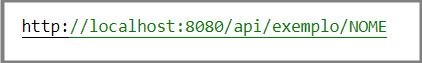
\includegraphics[width=0.40\textwidth]{./img/Endereço.png}
    \caption{URL de Acesso}
    \label{fig:Endereço}
    \end{figure}
    
    Como demostrado por \citen{souza} a \textit{@PathVariable} serve para obter um valor passado na URL. Seguindo o mapeamento do exemplo acima, basta executar a aplicação e acessar a seguinte URL para testar o controller.


\section{Angular 12 - Framework}

    O \textit{framework} que será utilizado é o \textit{Angular 12}, plataforma de aplicativo \textit{web, front-end} e de código aberto, a versão de produção mais recente, baseada em \textit{TypeScript} da empresa \textit{Google}. Segundo \citen{angular} o angular é uma plataforma \textit{evergreen}, o que significa que ela se mantém atualizada com o ecossistema em evolução da \textit{web}. A remoção de suporte a navegadores legados é permitido concentrar os esforços em fornecer soluções modernas e melhor suporte aos desenvolvedores e usuários.

    De acordo com \citen{nodejs} projeto aqui desenvolvido utiliza como padrão o \textit{Agular 12}, tendo ele como requisito ao menos a versão 10 do \textit{NodeJS}, portanto será necessário instalar a versão \textit{NodeJS 10} ou superior. Sendo o \textit{Node.js} um \textit{software} de código aberto, multiplataforma, baseado no interpretador V8 do \textit{Google} e que permite a execução de códigos \textit{JavaScript} fora de um navegador \textit{web}.
    
    Serão utilizadas as seguintes bibliotecas de extensões para o \textit{JavaScript}:
    
\begin{itemize}

    \item \textit{RxJS}, é uma biblioteca para programação reativa que possibilita o uso da programação para a linguagem de \textit{Java}, sendo uma biblioteca para compor programas assíncronos e baseados em eventos usando sequências \textit{Observables} \cite{rxjs};
    
     \item \textit{Moment.js}, é um pacote \textit{open source} que pode ser utilizado para validar, manipular e fazer o \textit{parse} de datas, definindo assim os valores de data baseados em \textit{string} no  \textit{JavaScript} \cite{moment}.

\end{itemize}

    Também será utilizado o \textit{Angular Material} como abordado por \citen{material} os componentes do \textit{material design} para o \textit{Angular}, possuindo-o alta qualidade com componentes internacionalizados e acessíveis para todos, bem testado para garantir desempenho e confiabilidade. Com \textit{APIs} simples, com comportamento consistente entre plataformas. Versátil, para fornece ferramentas que ajudam os desenvolvedores a construir seus próprios componentes personalizados com padrões de interação comuns e customizável dentro dos limites da especificação do \textit{Material Design}.
    
        \begin{figure}[h]
        \centering
        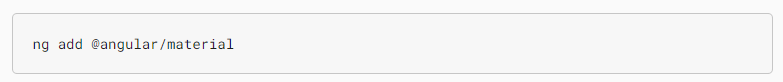
\includegraphics[width=0.70\textwidth]{./img/MaterialDesign.png}
        \caption{Exemplo de como adicionar a dependencia do Angular Material disponivel em \cite{material}.}
        \label{fig:MaterialDesign}
        \end{figure}


\section{Banco de Dados}
    Segundo \citen{dev}, um banco de dados é uma coleção de dados inter-relacionados, representando informações sobre um domínio específico, ou seja, sempre que for possível agrupar informações que se relacionam e tratam de um mesmo assunto, pode-se dizer que existe um banco de dados.
    
    A fim de estruturar o banco de dados será constituído a estrutura de tabelas conforme demostrado diagrama de entidade relacional. O modelo conceitual abaixo demostra os relacionamentos de avalição feito para um docente do Instituto Federal de Goiás e apresenta um diagrama de entidade relacionamento, em que são identificados os relacionamentos entre as entidade, sua cardinalidades. Também são apresentados para cada entidade suas chaves primarias e secundarias bem como seus dados.
    
    \begin{figure}[h]
    \centering
    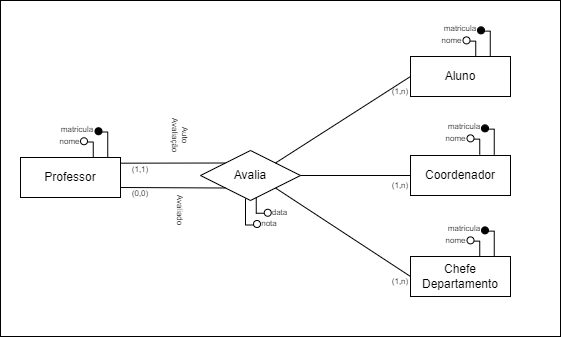
\includegraphics[width=0.72\textwidth]{./img/ModeloEntidadeRelacionamento.png}
    \caption{Diagrama de Entidade Relacionamento}
    \label{fig:ModeloEntidadeRelacionamento}
    \end{figure}

    Conforme evidenciado por \citen{mer} foi desenvolvido o diagrama de entidade relacional para facilitar o projeto logico do banco de dados, permitindo a representação da estruturação lógica, sendo um dos modelos de dados com maior capacidade semântica e representa um problema como um conjunto de entidades e relacionamentos entre estas entidades.

    O banco de dados que utilizado no projeto, será o \textit{SQL Serve 2017}, segundo a \citen{microsoft},  \textit{SQL Server 2017} Express é um sistema gratuito de gerenciamento de dados avançado e confiável, que fornece um repositório de dados para sites leves e aplicativos de área de trabalho. 

    A abordagem pensada está visando desempenho do banco de dados, será criado uma zona segura de processamento seguindo um padrão de escalar verticalmente, refere-se à quantidade que pode ser consumida sem atingir o limite de saturação. Neste cenário, a zona segura é considerada ao respeitar a quantidade de recursos estipulada, ou utilizando até 60\% de CPU.
   
    \begin{figure}[h]
    \centering
    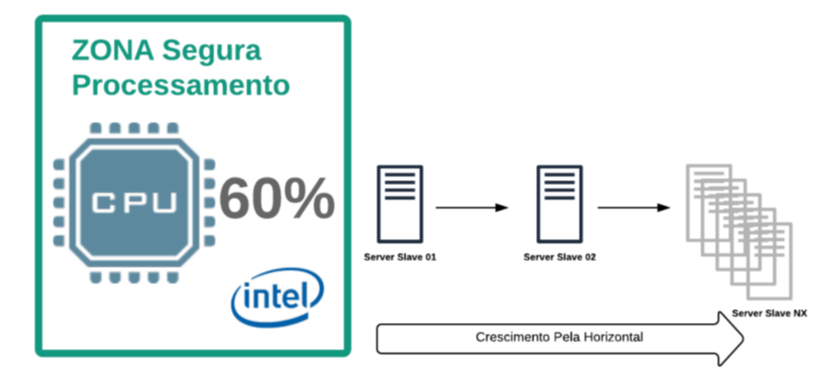
\includegraphics[width=0.75\textwidth]{./img/segProc.png}
    \caption{Modelo de Implementação do Banco de Dados \citen{totvs}}
    \label{fig:segProc}
    \end{figure}

    Uma das recomendação a ser seguida no momento da implantação do SAD, no \textit{hardware} físico indicado para uma melhor performance, o uso de volumes \textit{High Perfomance} (como \textit{SSD/Flash}), considerando a volumetria/conexões do ambiente.    
    
    
\section{Abordagens de Testes de Usabilidade e Desempenho do Sistema}

    Baseado nos requisitos levantados juntamente com a Comissão Permanente de Pessoal Docente, será desenvolvido o Sistema para Avaliação de Desempenho Docente, e para efetuação dos testes de desempenho e usabilidade do sistema, serão desenvolvidas algumas abordagens para concretização do projeto.
    
    Segundo \citen{patel} teste de usabilidade é um método de verificação de funcionalidades da interface de uma plataforma digital. É empregado em websites, aplicações e outras ferramentas, levando usuários reais à execução de determinadas tarefas. Após sua realização, é realizada uma análise de usabilidade e das principais dificuldades.
    
    Conforme abordado por \citen{desempenho} o teste de desempenho é uma classe de testes implementada e executada para caracterizar e avaliar as características relacionadas ao desempenho do destino do teste, como perfis de sincronização, fluxo de execução, tempos de resposta e confiabilidade e limites operacionais. 
    
    Portanto, ao realizar o teste enxergará a interface do ponto de vista de que a utilizará. Será efetuado o modelos de teste que visa a descoberta de problemas, esse modelo de teste quando aplicado, seu objetivo é identificar e corrigir eventuais problemas existentes na aplicação, observando quais são os obstáculos para a fluida utilização.
    
    Existirá numa primeira etapa a efetuação dos testes de aceitação juntamente com os integrantes da CPPD, com um protótipo já elaborado serão efetuadas abordagens de aceitação juntamente com alguns docentes e alunos, elaborando um processo de avaliação de desempenho. Essa avaliação será preenchida, e a partir deste preenchimento poderá avaliar se os dados gerados conseguiram atender a demanda esperada e se o desempenho e usabilidade do software necessitará de ajustes.


    %  Teste de aceitação com pessoal da CPPD 10 professor e alunos
 
